\section{Software Testing}\label{s:TestingFrameworkTheory}

\paragraph{Idea:} \emph{Reuse LSTS toolchain architecture} for DAA testing framework.

\paragraph{LSTS Toolchain:} Software architecture used in modern unmanned aerial vehicles must be system independent and scalable. Writing own control software for unmanned aerial vehicle and ground station is unthinkable in the current state of the art.  Most notable framework for unmanned aerial vehicle development is the LSTS toolchain from University of Porto \cite{merani2011underwater}. This toolchain is widespread in other universities, and multiple independent applications are based on it \cite{rajan2013towards}.

\begin{figure}[H]
    \centering
    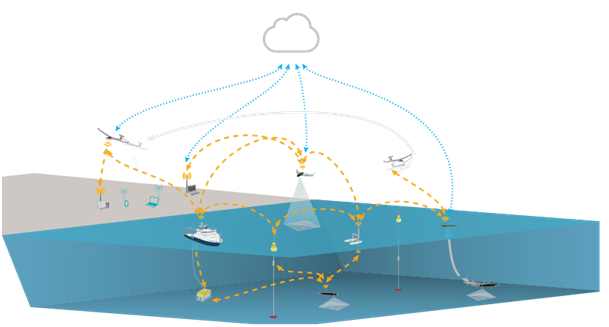
\includegraphics[width=0.9\linewidth]{\FIGDIR/TE036LSTSDeployment}
    \caption{Example of LSTS toolchain deployment in a real environment \cite{pinto2006neptus}}
    \label{fig:lstsdeployment}
\end{figure}

Example of software architecture implementation is shown in figure \ref{fig:lstsdeployment} LSTS HUB (cloud iconography) is collecting all important data from currently executing missions. Data are transferred via REST API (dotted blue lines) to HUB.  Commanded vehicles can be unmanned copters, planes, ships, submarines or floating sensors compounds. Each vehicle has installed DUNE which is responsible for vehicle command and ground control station communication. Deployment, a range of command and status messages can vary. The ground station can be implemented on a personal computer (any platform) in NEPTUS environment or mobile platform (Android OS) in ACCU environment. Ground station environments are customizable and open source. The layout of the ground station can be customized to need of current mission via plugins or console configuration. Vehicles and ground stations are communicating via IMC protocol (orange dashed lines). The communication channel is platform independent.


\textit{Glued} is a Debian-based open source operating system which was initially released in 2010.  Over the years it has become fairly widespread and been provided continuous updates.  Meanwhile, a notable development community has emerged, where advice and support can be received as more applications are investigated. Some of the merits of the operating system are its reliability and customizability. Operation system is developed for unmanned autonomous vehicles. It is widely used in air, sea and land vehicles. Customization allows the operating system to be tailored to the specific usage. For this purpose, this includes stripping off functionality which is not required, thus releasing resources to be focused on the essential tasks. Glued is the operating system favored by the Beaglebone development community, and thus there exist considerable amounts of helpful documentation for this set-up.

\textit{DUNE: Unified Navigational Environment} is an onboard software solution for unmanned vehicles. Multiple applications already run on this software. Almost any extension can be added to this to this environment. The software solution provides a means for interacting with the connected components as well as control, navigation, supervision and plan execution.  It is both CPU architecture independent and OS independent.  It is written in C++ and developed by LSTS: Underwater Systems and Technology Laboratory.

\textit{Neptus} \cite{pinto2006neptus,dias2006mission,dias2005neptus} is a command and control software operated from a ground station. It is designed to operate well together with Dune and was also developed by LSTS. Neptus provides tools for remotely monitoring UAVs and assigning plans and commands in real-time missions, supporting multiple connections dynamically. Furthermore, it provides possibilities for both simulating missions and reviewing previously performed operations. This is presented in a customizable interface equipped with map layers and control panels. It is written in Java and available for both Windows and Linux systems.

The \textit{Inter-Module Communication} \cite{martins2009imc} (IMC) protocol was developed by LSTS to provide reliable communication between the systems.  The protocol is message-oriented, such that messages can be sent and received from a bus which connects independently run threads or systems.  Thus it functions as a method of communication between tasks internally in Dune, and can also be passed to and from other vehicles or computers running Dune or Neptus.  IMC is platform independent at multiple messages have been already developed and supported by both DUNE and Neptus (around 400 status/command messages).

\textit{HUB} is communication hub for data dissemination and situation awareness. This module is responsible for complex mission execution when cooperation of multiple pilots/vehicles is required. This module can be imagined as an airport tower (traffic control) center, which is monitoring all flights in the airport (operation site) area.

\paragraph{Movement Automaton Control} Marconi used \emph{hybrid automaton} with forced \emph{State Switch} via buffer \cite{marconi2009control}. The key concept is that \emph{Automata} state switch is forced as \emph{external source command}. Our \emph{Movement Automaton} implementation knows only \emph{forced state switch} like in \cite{frazzoli2000trajectory}. 

\paragraph{Used concepts:} Most of the architecture was re-used in our approach, the concept of \emph{Rule engine} (sec. \ref{sec:ruleEngine}) was introduced to cover missing \emph{UTM} related functionality. The implementation in Matlab was influenced by Alessandeti works \cite{allesandeti2016virtualArena,alessandrettinotes}. The other aircraft dynamic and control related concepts were taken from  \cite{stevens2015aircraft}.

